\section{Evaluation}
\label{section:evaluation}

In order to evaluate the scalability of our subsetter we performed strong
scaling tests.  All tests were performed on the franklin Cray-XT4
supercomputer\cite{franklin} located at NERSC\cite{NERSC}.  The performance
data collected was generated by custom wrappers to the functions we developed.
The IO wrappers perform barriers before and after each collective IO operation
is called with the start and end timestamps collected immediately after each
barrier using \verb=clock_gettime()= or \verb=gettimeofday()= depending on
platform availability.  Before program termination, the number of bytes
written and read and the total time spent performing IO is collected on the
zeroth process and displayed in terms of GB/s.  The profiling information
collects the number of times each function is called and how much time was
spent in each function.  It is only reported for the zeroth process and is
meant only as a general measure of performance.  The IO and function profile
data were collected on separate runs so that the collection of one would not
affect the other.

\subsection{Strong Scaling}

\begin{figure}[!t]
\center
\resizebox{3.5in}{!}{
% GNUPLOT: LaTeX picture with Postscript
\begingroup
  \makeatletter
  \providecommand\color[2][]{%
    \GenericError{(gnuplot) \space\space\space\@spaces}{%
      Package color not loaded in conjunction with
      terminal option `colourtext'%
    }{See the gnuplot documentation for explanation.%
    }{Either use 'blacktext' in gnuplot or load the package
      color.sty in LaTeX.}%
    \renewcommand\color[2][]{}%
  }%
  \providecommand\includegraphics[2][]{%
    \GenericError{(gnuplot) \space\space\space\@spaces}{%
      Package graphicx or graphics not loaded%
    }{See the gnuplot documentation for explanation.%
    }{The gnuplot epslatex terminal needs graphicx.sty or graphics.sty.}%
    \renewcommand\includegraphics[2][]{}%
  }%
  \providecommand\rotatebox[2]{#2}%
  \@ifundefined{ifGPcolor}{%
    \newif\ifGPcolor
    \GPcolortrue
  }{}%
  \@ifundefined{ifGPblacktext}{%
    \newif\ifGPblacktext
    \GPblacktexttrue
  }{}%
  % define a \g@addto@macro without @ in the name:
  \let\gplgaddtomacro\g@addto@macro
  % define empty templates for all commands taking text:
  \gdef\gplbacktext{}%
  \gdef\gplfronttext{}%
  \makeatother
  \ifGPblacktext
    % no textcolor at all
    \def\colorrgb#1{}%
    \def\colorgray#1{}%
  \else
    % gray or color?
    \ifGPcolor
      \def\colorrgb#1{\color[rgb]{#1}}%
      \def\colorgray#1{\color[gray]{#1}}%
      \expandafter\def\csname LTw\endcsname{\color{white}}%
      \expandafter\def\csname LTb\endcsname{\color{black}}%
      \expandafter\def\csname LTa\endcsname{\color{black}}%
      \expandafter\def\csname LT0\endcsname{\color[rgb]{1,0,0}}%
      \expandafter\def\csname LT1\endcsname{\color[rgb]{0,1,0}}%
      \expandafter\def\csname LT2\endcsname{\color[rgb]{0,0,1}}%
      \expandafter\def\csname LT3\endcsname{\color[rgb]{1,0,1}}%
      \expandafter\def\csname LT4\endcsname{\color[rgb]{0,1,1}}%
      \expandafter\def\csname LT5\endcsname{\color[rgb]{1,1,0}}%
      \expandafter\def\csname LT6\endcsname{\color[rgb]{0,0,0}}%
      \expandafter\def\csname LT7\endcsname{\color[rgb]{1,0.3,0}}%
      \expandafter\def\csname LT8\endcsname{\color[rgb]{0.5,0.5,0.5}}%
    \else
      % gray
      \def\colorrgb#1{\color{black}}%
      \def\colorgray#1{\color[gray]{#1}}%
      \expandafter\def\csname LTw\endcsname{\color{white}}%
      \expandafter\def\csname LTb\endcsname{\color{black}}%
      \expandafter\def\csname LTa\endcsname{\color{black}}%
      \expandafter\def\csname LT0\endcsname{\color{black}}%
      \expandafter\def\csname LT1\endcsname{\color{black}}%
      \expandafter\def\csname LT2\endcsname{\color{black}}%
      \expandafter\def\csname LT3\endcsname{\color{black}}%
      \expandafter\def\csname LT4\endcsname{\color{black}}%
      \expandafter\def\csname LT5\endcsname{\color{black}}%
      \expandafter\def\csname LT6\endcsname{\color{black}}%
      \expandafter\def\csname LT7\endcsname{\color{black}}%
      \expandafter\def\csname LT8\endcsname{\color{black}}%
    \fi
  \fi
  \setlength{\unitlength}{0.0500bp}%
  \begin{picture}(7200.00,5040.00)%
    \gplgaddtomacro\gplbacktext{%
      \csname LTb\endcsname%
      \put(1342,704){\makebox(0,0)[r]{\strut{} 100}}%
      \put(1342,4380){\makebox(0,0)[r]{\strut{} 1000}}%
      \put(1474,484){\makebox(0,0){\strut{} 64}}%
      \put(2553,484){\makebox(0,0){\strut{} 128}}%
      \put(3632,484){\makebox(0,0){\strut{} 256}}%
      \put(4712,484){\makebox(0,0){\strut{} 512}}%
      \put(5791,484){\makebox(0,0){\strut{} 1024}}%
      \put(6870,484){\makebox(0,0){\strut{} 2048}}%
      \put(440,2542){\rotatebox{90}{\makebox(0,0){\strut{}Time (s)}}}%
      \put(4172,154){\makebox(0,0){\strut{}Cores}}%
      \put(4172,4710){\makebox(0,0){\strut{}Strong Scaling Test}}%
    }%
    \gplgaddtomacro\gplfronttext{%
      \csname LTb\endcsname%
      \put(5883,4207){\makebox(0,0)[r]{\strut{}Cores:Time}}%
    }%
    \gplbacktext
    \put(0,0){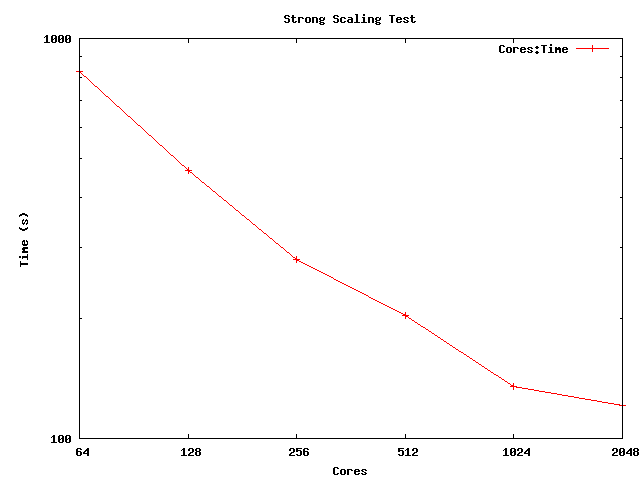
\includegraphics{strong}}%
    \gplfronttext
  \end{picture}%
\endgroup

}
\caption{Strong Scaling Test}
\label{fig:strong}
\end{figure}

\begin{figure}[!t]
\center
\resizebox{3.5in}{!}{
% GNUPLOT: LaTeX picture with Postscript
\begingroup
  \makeatletter
  \providecommand\color[2][]{%
    \GenericError{(gnuplot) \space\space\space\@spaces}{%
      Package color not loaded in conjunction with
      terminal option `colourtext'%
    }{See the gnuplot documentation for explanation.%
    }{Either use 'blacktext' in gnuplot or load the package
      color.sty in LaTeX.}%
    \renewcommand\color[2][]{}%
  }%
  \providecommand\includegraphics[2][]{%
    \GenericError{(gnuplot) \space\space\space\@spaces}{%
      Package graphicx or graphics not loaded%
    }{See the gnuplot documentation for explanation.%
    }{The gnuplot epslatex terminal needs graphicx.sty or graphics.sty.}%
    \renewcommand\includegraphics[2][]{}%
  }%
  \providecommand\rotatebox[2]{#2}%
  \@ifundefined{ifGPcolor}{%
    \newif\ifGPcolor
    \GPcolortrue
  }{}%
  \@ifundefined{ifGPblacktext}{%
    \newif\ifGPblacktext
    \GPblacktexttrue
  }{}%
  % define a \g@addto@macro without @ in the name:
  \let\gplgaddtomacro\g@addto@macro
  % define empty templates for all commands taking text:
  \gdef\gplbacktext{}%
  \gdef\gplfronttext{}%
  \makeatother
  \ifGPblacktext
    % no textcolor at all
    \def\colorrgb#1{}%
    \def\colorgray#1{}%
  \else
    % gray or color?
    \ifGPcolor
      \def\colorrgb#1{\color[rgb]{#1}}%
      \def\colorgray#1{\color[gray]{#1}}%
      \expandafter\def\csname LTw\endcsname{\color{white}}%
      \expandafter\def\csname LTb\endcsname{\color{black}}%
      \expandafter\def\csname LTa\endcsname{\color{black}}%
      \expandafter\def\csname LT0\endcsname{\color[rgb]{1,0,0}}%
      \expandafter\def\csname LT1\endcsname{\color[rgb]{0,1,0}}%
      \expandafter\def\csname LT2\endcsname{\color[rgb]{0,0,1}}%
      \expandafter\def\csname LT3\endcsname{\color[rgb]{1,0,1}}%
      \expandafter\def\csname LT4\endcsname{\color[rgb]{0,1,1}}%
      \expandafter\def\csname LT5\endcsname{\color[rgb]{1,1,0}}%
      \expandafter\def\csname LT6\endcsname{\color[rgb]{0,0,0}}%
      \expandafter\def\csname LT7\endcsname{\color[rgb]{1,0.3,0}}%
      \expandafter\def\csname LT8\endcsname{\color[rgb]{0.5,0.5,0.5}}%
    \else
      % gray
      \def\colorrgb#1{\color{black}}%
      \def\colorgray#1{\color[gray]{#1}}%
      \expandafter\def\csname LTw\endcsname{\color{white}}%
      \expandafter\def\csname LTb\endcsname{\color{black}}%
      \expandafter\def\csname LTa\endcsname{\color{black}}%
      \expandafter\def\csname LT0\endcsname{\color{black}}%
      \expandafter\def\csname LT1\endcsname{\color{black}}%
      \expandafter\def\csname LT2\endcsname{\color{black}}%
      \expandafter\def\csname LT3\endcsname{\color{black}}%
      \expandafter\def\csname LT4\endcsname{\color{black}}%
      \expandafter\def\csname LT5\endcsname{\color{black}}%
      \expandafter\def\csname LT6\endcsname{\color{black}}%
      \expandafter\def\csname LT7\endcsname{\color{black}}%
      \expandafter\def\csname LT8\endcsname{\color{black}}%
    \fi
  \fi
  \setlength{\unitlength}{0.0500bp}%
  \begin{picture}(7200.00,5040.00)%
    \gplgaddtomacro\gplbacktext{%
      \csname LTb\endcsname%
      \put(990,660){\makebox(0,0)[r]{\strut{} 0}}%
      \put(990,1032){\makebox(0,0)[r]{\strut{} 0.5}}%
      \put(990,1404){\makebox(0,0)[r]{\strut{} 1}}%
      \put(990,1776){\makebox(0,0)[r]{\strut{} 1.5}}%
      \put(990,2148){\makebox(0,0)[r]{\strut{} 2}}%
      \put(990,2520){\makebox(0,0)[r]{\strut{} 2.5}}%
      \put(990,2892){\makebox(0,0)[r]{\strut{} 3}}%
      \put(990,3264){\makebox(0,0)[r]{\strut{} 3.5}}%
      \put(990,3636){\makebox(0,0)[r]{\strut{} 4}}%
      \put(990,4008){\makebox(0,0)[r]{\strut{} 4.5}}%
      \put(990,4380){\makebox(0,0)[r]{\strut{} 5}}%
      \put(1122,440){\makebox(0,0){\strut{} 64}}%
      \put(2263,440){\makebox(0,0){\strut{} 128}}%
      \put(3404,440){\makebox(0,0){\strut{} 256}}%
      \put(4544,440){\makebox(0,0){\strut{} 512}}%
      \put(5685,440){\makebox(0,0){\strut{} 1024}}%
      \put(6826,440){\makebox(0,0){\strut{} 2048}}%
      \put(220,2520){\rotatebox{90}{\makebox(0,0){\strut{}Bandwidth (GB/s)}}}%
      \put(3974,110){\makebox(0,0){\strut{}Cores}}%
      \put(3974,4710){\makebox(0,0){\strut{}Strong Scaling - IO - 48 OSTs}}%
    }%
    \gplgaddtomacro\gplfronttext{%
      \csname LTb\endcsname%
      \put(5839,4207){\makebox(0,0)[r]{\strut{}Read}}%
      \csname LTb\endcsname%
      \put(5839,3987){\makebox(0,0)[r]{\strut{}Write}}%
    }%
    \gplbacktext
    \put(0,0){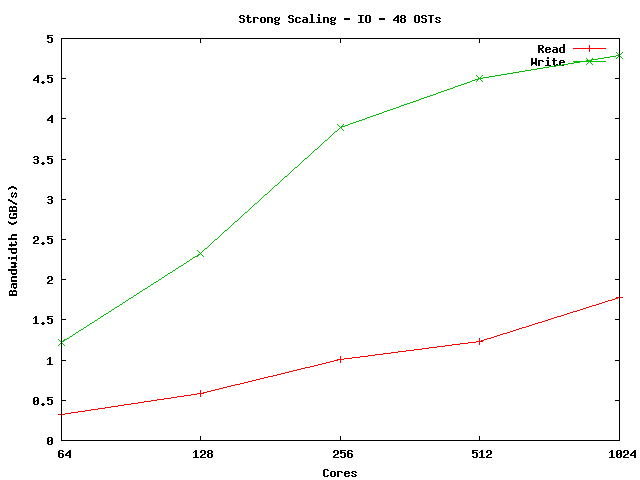
\includegraphics{strong_io}}%
    \gplfronttext
  \end{picture}%
\endgroup

}
\caption{Strong Scaling Test - IO}
\label{fig:strong_io}
\end{figure}

\begin{table*}[!t]
\center
\caption{Strong Scaling Profile for Process 0}
\label{tab:strong_prof}
\begin{tabular}{lllllll}
Name&Calls&Prcnt&Times&Prcnt&T/call&Prcnt\\
NetcdfVariable::read()&39&0.1&47710000&0.79&1223333.3&79.5\\
NetcdfFileWriter::write(int,int,int)&34&0.1&8460000&0.14&248823.5&14.1\\
ConnectivityVariable::reindex()&3&0&1480000&0.02&493333.3&2.5\\
VariableDecorator::read()&5&0&780000&0.01&156000&1.3\\
NetcdfDataset::NetcdfDataset(string)&5&0&670000&0.01&134000&1.1\\
Dataset::adjust\_masks(LatLonBox)&1&0&600000&0.01&600000&1\\
%NetcdfFileWriter::NetcdfFileWriter(string)&1&0&180000&0&180000&0.3\\
%AbstractVariable::get\_handle()&165&0.3&140000&0&848.5&0.2\\
%pack(int,int,int*,int*)&31&0.1&70000&0&2258.1&0.1\\
%NetcdfFileWriter::maybe\_enddef()&68&0.1&60000&0&882.4&0.1\\
%Dataset::create\_masks()&1&0&50000&0&50000&0.1\\
%LatLonBox::contains(double,double)&40961&78&40000&0&1&0.1\\
%AbstractVariable::release\_handle()&50&0.1&20000&0&400&0\\
%AggregationVariable::release\_handle()&2&0&10000&0&5000&0\\
\end{tabular}
\end{table*}

This test was run over 24 timesteps of an edge variable at a 4Km resolution
(R=11) specifying a subset region of the Madden-Julien Oscillation\cite{MJO}
(20N,-20S,160E,90E).  One timestep of the edge variable is 12.1875 GB.  Figure
\ref{fig:strong} shows the timing results of the test while Figure
\ref{fig:strong_io} shows the IO bandwidth.  The number of processors was
doubled each run starting from 64.

Table \ref{tab:strong_prof} is a table of a profile for process zero for the
1024 process run.  The function names are sufficiently self-documenting for
those familiar with C++ syntax.  The zeroth process represents a worst-case
scenario since the default distribution of data using GA will always put data
on at least the zeroth process implying process zero should have at least as
much work to perform as any other processor.  The profile for the 1024 run was
selected arbitrarily, however the profiles for the other strong scaling runs
demonstrated a similar trend.

Although initially promsing at scales of over 2000 cores, it is not entirely
clear that the algorithms we have developed are sufficient due to the large
mismatch between IO and everything else.  The profile suggests that IO
accounts for nearly 85\% of program execution.  This is not a stretch of the
imagination since our software merely reads, subsets, and writes.  Even if our
code performed a significant calculation after each read of the edge variable,
the profile would likely remain IO bound but less so.

The reason for the disproportionately faster write bandwidth versus read
bandwith is likely due to caching by the Lustre filesystem.  The relatively
small amount of data being written is likely being copied to an internal
buffer allowing the functions to return rather quickly.  Furthermore, there is
ongoing work to allow the subsetter program to read in a less substantial
amount of data based on the desired subset.  As it is now, the subsetter reads
the entire horizontal domain and immediately culls what falls outside of the
specified region.  For example, the MJO region is roughly 6.5\% of the global
data.  An idea worth further research would be to implement a collective read
routine similar to the one-sided \verb+NGA_Gather+ provided by GA.

%\subsection{Weak Scaling}

%\begin{figure}[!t]
%\center
%\resizebox{3.5in}{!}{
%TODO - FIGURE
%%\input{plots/weak}
%}
%\caption{Weak Scaling Test}
%\label{fig:weak}
%\end{figure}

%\begin{figure}[!t]
%\center
%\resizebox{3.5in}{!}{
%TODO - FIGURE
%%\input{plots/weak_io}
%}
%\caption{Weak Scaling Test - IO}
%\label{fig:weak_io}
%\end{figure}

%\begin{figure*}[!t]
%\center
%\begin{tabular}{lllllll}
%Name&Calls&Prcnt&Times&Prcnt&T/call&Prcnt\\
%TODO&TODO&TODO&TODO&TODO&TODO&TODO\\
%\end{tabular}
%\caption{Weak Scaling Profile for Process 0}
%\label{fig:weak_prof}
%\end{figure*}

%This test was run over 24 timesteps while varying both the number of
%processors as well as the resolution of the model, affecting the amount of
%data processed.  Figure \ref{fig:weak} shows the timing results of the test
%while Figure \ref{fig:weak_io} shows the IO bandwidth.  The number of
%processors as well as the model resolution was doubled for each run starting
%from 16 processors at a model resolution of 125Km through 512 processors at a
%model resolution of 4Km.
